% main.tex

% To enable the camera-ready format, use the following line
%\documentclass{gtac}

% To enable the double-blind submission format for the review process, use the following line

\documentclass[11pt, onecolumn, journal,compsoc]{IEEEtran}

\usepackage{graphicx}
\usepackage{tikz}
\usetikzlibrary{matrix,calc}
\usepackage{pgfplots}
\usepackage{cite}
\usepackage{bm}
\usepackage{url}
\usepackage{breqn}
\usepackage{diagbox}
\usepackage{float}
\usepackage{xcolor}
\usepackage{mathtools}
\usepackage{amsthm}
\usepackage{amsthm}
\usepackage{amsfonts}
\usepackage{amssymb}
\usepackage{times}
\usepackage{hyperref}
\usepackage{cleveref}
\usepackage{flushend}
\usepackage{algorithm}
\usepackage{algpseudocode}
\usepackage{soul}
\usepackage[export]{adjustbox}
\usepackage{subfig}
\usepackage{preview}
\usepackage{pifont}

\renewcommand{\algorithmicrequire}{\textbf{Input:}}
\renewcommand{\algorithmicensure}{\textbf{Output:}}

\newcounter{pgfcurrentmatrix}

\newcommand{\Plus}{\mathord{\begin{tikzpicture}[baseline=0ex, line width=1, scale=0.13]
  \draw (1,0) -- (1,2);
  \draw (0,1) -- (2,1);
  \end{tikzpicture}}}

% Used in the matlab2tikz package
\newlength\figureheight 
\newlength\figurewidth 

\newtheoremstyle{problemstyle}  % <name>
        {8pt}                                               % <space above>
        {8pt}                                               % <space below>
        {\normalfont}                               % <body font>
        {}                                                  % <indent amount}
        {\bfseries\itshape}                 % <theorem head font>
        {\normalfont\bfseries:}         % <punctuation after theorem head>
        {.5em}                                          % <space after theorem head>
        {}                                                  % <theorem head spec (can be left empty, meaning `normal')>
\theoremstyle{problemstyle}

\newtheorem{problem}{Problem}%[section]

\title{Partial Radix Passes for Improved Performance in rocFFT}
\author{Flavio Teixeira, Malcolm Roberts \\
AI GPU Software (AGS) \\
flavio.teixeira,malcolm.roberts@amd.com} % Adjust the author names here


\begin{document}

\maketitle % Create the title section

\begin{abstract}

We present a new method to optimally distribute FFT work among compute
kernels based on the amount of available shared memory. Rearranging
FFT work in this fashion allow us to reduce the total number of passes
through global memory, which is frequently the bottleneck in GPU-based
FFT algorithms. For rocFFT, the software library for computing FFTs in
AMD's ROCm ecosystem, the reduction in global memory transactions
directly translates to improved performance for many HPC and ML
customers critical workloads.  As far as we are able to tell, this
technique is novel, and is not observed in other FFT libraries.

\end{abstract}

%\keywords{Fast Fourier Transforms, High Performance Computing, GPU Algorithms, Numerical Optimization}

\section{Introduction}

The Fast Fourier Transform (FFT) is widely considered one of the most influential algorithms in science and engineering \cite{garravan00}. It is the most ubiquitous algorithm for processing digital or discrete data. The FFT is also used in many other disciplines including music, mathematics, and economics. An example of FFTs applied to probabilistic dimensionality reduction methods for machine learning can be found in \cite{nasseira20}.

Compute continues to outpace memory bandwidth in every new GPU
generation. Since the arithmetic intensity of FFTs are not high and
there is an imbalance between compute and memory bandwidth in modern GPU
architectures, the performance of FFTs is heavily dependent on the
memory subsystem. If $N$ is a power of 2, then a radix-$2$ FFT
algorithm recursively expresses the one-dimensional Discrete Fourier
Transform (DFT) of length-$N$ in terms of smaller DFTs of length
$N/2$. For GPU-based FFT algorithms, the small DFTs in each recursion
or pass of the FFT are performed entirely in shared-memory for
improved performance, while the bottleneck is usually the global
memory. A single round-trip to global memory is required when $N$ is
small, but for large enough $N$ an hierarchical algorithm that entails
several passes through global memory is required. Multidimensional
FFTs have similar compute and memory requirements.

\textbf{Main Results:} In this work, we present a method to optimally
distribute FFT work among the compute kernels based on the amount of
available shared memory. This method is shown to be applicable to many
GPU-based FFT compute schemes, including large one-dimensional and
multidimensional FFTs. We then focus on the multidimensional case, and
show that by performing partial radix passes in a compute kernel
off-dimension in 3D FFTs, the total number of
round-trips to global memory is reduce by one-third. Theoretical results are complemented with numerical experiments, which demonstrate significantly improved performance of the proposed method on molecular dynamics simulation workloads.
%TODO: Add numerical results here.

\section{Background}

Before presenting the proposed method, we first review the one-dimensional and multi-dimensional DFT equations. We then proceed to a brief review of FFT algorithms and discuss implementation details of FFTs on GPUs. We finish this section describing a well-known decomposition of FFT work that will serve as a foundation for the proposed method. 
\subsection{Discrete Fourier Transform}
Let $\bm{y} = \mathcal{F}\left\{ \bm{x} \right\}$ denote the one-dimensional DFT of $\bm{x}$, which maps an $N$-length input sequence $\bm{x} = \begin{bmatrix} x_0 &  \cdots & x_{N-1} \end{bmatrix}$ into an $N$-length output sequence $\bm{y} = \begin{bmatrix} y_0 & \cdots & y_{N-1} \end{bmatrix}$ with
\begin{equation}
y_k = \sum_{n=0}^{N-1}{x_n e^{-\frac{2 \pi \jmath}{N}nk}}, \qquad k = 0, \ \ldots, \ N-1.
\label{eq:dft}
\end{equation}
The DFT can also be expressed in matrix form as $\bm{y} = \bm{F}_N \bm{x}$, where $\bm{F}_N$ is the $N \times N$ DFT matrix with entries $F_{n,k} = \exp (\frac{-2\pi \jmath}{N} nk )$.

For the multidimensional case, let $d$ denote the number of dimensions with $N=N_1 \times \cdots \times N_d$. If we treat the $N$-length input and output sequences $\bm{x}$ and $\bm{y}$ as $d$-dimensional arrays as $\bm{x} \coloneq \bm{x}(0 \colon N_1-1,\ 0 \colon N_2-1, \ \cdots,\ 0 \colon N_d-1)$ and $\bm{y} \coloneq \bm{y}(0 \colon N_1-1,\ 0\colon N_2-1, \ \cdots,\ 0 \colon N_d-1)$, where the notation $(0 \colon N)$ is used for index vectors, i.e., $\bm{i}$ is an index vector, such that $\bm{i}=0 \colon N \ \Leftrightarrow \ \bm{i}=\begin{bmatrix} 0 & 1 & \cdots & N-1 \end{bmatrix}$, then the $d$-dimensional DFT is defined as
\begin{equation}
y_{k_1, \cdots, k_d} = \sum_{n_1=0}^{N_1-1}{\cdots}\sum_{n_d=0}^{N_d-1}{x_{n_1 \cdots n_d} e^{-\frac{2 \pi \jmath}{N}n_1k_1} \cdots e^{-\frac{2 \pi \jmath}{N}n_d k_d}}
\label{eq:multi_dimdft}
\end{equation}

In this work, we focus on complex-valued entries for the input and output sequences. 
\subsection{Mixed-Radix FFTs}
The FFT is a family of algorithms for computing the DFT in $O(N \log(N))$. FFTs are significantly faster than the DFT which scales as $O(N^2)$. To achieve reduced computational complexity, these algorithms use a divide-and-conquer approach for the computation of the DFT. For example, if $N$ is a power of $2$, then the summation in \labelcref{eq:dft} can be split into two smaller summations in $N/2$, one with the even entries, and the other with the odd entries of the input sequence. Applying this splitting rule to \labelcref{eq:dft} is equivalent to computing two smaller DFTs of length-$N/2$. This procedure can in turn be applied recursively to the smaller summations until a length-$2$ DFT is reached. This is the essence of the radix-$2$ Cooley-Tukey (C-T) FFT algorithm. Each recursion of the splitting rule is also known as a stage or a pass of the FFT. There are $\log(N)$ stages for a radix-$2$ FFT and $N/2$ length-$2$ DFTs to be performed at each stage.	

More generally, if $N$ is highly composite, e.g., $N=q_1 \times q_2 \times \cdots \times q_k$, then the summation in \labelcref{eq:dft} can be recursively split into smaller summations, starting with $q_1$ summations in $N/q_1$. These summations in turn can then be split into $q_2$ summations in $N/q_2$, and so on. This procedure corresponds to a mixed-radix C-T algorithm \cite{vanloan92}. There are $k$ stages or passes in a mixed-radix FFT with $N=q_1 \times q_2 \times \cdots \times q_k$ and $N/q_i$ length-$q_i$ DFTs to be performed at each stage. 

\subsection{Computing FFTs with GPUs}

Each DFT in a given stage is completely independent from each other, thus the entire FFT work of a stage is parallelizable. Each stage requires writing intermediate results back to memory. Since global memory bandwidth is significantly lower than the GPU compute units bandwidth, the FFT passes or stages are performed entirely in shared memory. With this approach, only a single round-trip to global memory is required. The amount of available shared memory is, therefore, a determining factor for FFT performance in GPUs. FFTs are clearly memory bound workloads on these devices, since each DFT in an FFT stage typically has low arithmetic intensity.

The splitting rule in the C-T algorithm with even and odd entries of the input sequence requires an index-shuffling stage, which is equivalent to a bit-reversal of the input sequence indices in binary form, and that leads to incoherent memory accesses patterns. GPU implementations typically use a variation of C-T called the Stockham algorithm \cite{gonabrdoyusmma08}, which is similar to C-T with the exception of how the indices are arranged in each stage, leading to more favourable access patterns for GPUs.

From the definition in \labelcref{eq:multi_dimdft}, multidimensional DFTs are separable transforms, meaning that these transforms can be implemented by computing FFTs independently along each dimension. From an implementation point of view, higher dimensions suffer from unfavourable global memory access patterns, since large strides are required for consecutive elements in the working dimension. Consequently, GPU implementations usually interleave data transpositions between the FFT compute kernels, such that the highest dimension is moved down to the lowest dimension to avoid large strided accesses. Data transposition is fused into the FFT compute kernel whenever possible, such that global memory transactions are reduced.

\subsection{FFT Work Decomposition}

Consider the case where an FFT of length-$N$ does not fit into shared memory. If this FFT is to be performed entirely in global memory, then $\log(N)$ round-trips to global memory are required if a radix-$2$ implementation is used, or more generally, $k$ round-trips with $N=q_1 \times q_2 \times \cdots \times q_k$ if a mixed-radix FFT is carried out. This compute scheme, however, would be generally slow and inefficient on modern GPUs since global memory is significant slower than the compute units. 

We now describe a well-known procedure that allows a length-$N$ FFT to be decomposed into a series of smaller FFTs. Let $\bm{F}_N (0 \colon N_a-1, 0 \colon N_b-1)$ with $N = N_a \times N_b$ denote an $N_a \times N_b$ submatrix of the DFT matrix $\bm{F}_N$ obtained by picking the $0$ to $N_a-1$ rows and the $0$ to $N_b-1$ columns of $\bm{F}_N$. Similarly, let $\bm{X}_{N_a \times N_b}$ denote an $N_a \times N_b$ matrix obtained by a column major-ordering of $\bm{x}$, i.e., by picking every consecutive $N_a$ entries of $\bm{x}$ and setting them as columns of $\bm{X}_{N_a \times N_b}$. \Cref{alg:4_step_fft} define the steps for performing a large, length-$N$ FFT with $N = N_a \times N_b$, in terms of two smaller FFTs of length $N_a$ and $N_b$.
\begin{algorithm}
\begin{algorithmic}[1]
\State $\bm{X}_{N_a \times N_b} \gets \bm{X}_{N_a \times N_b} \bm{F}_{N_b}$ 
\State $\bm{X}_{N_a \times N_b} \gets \bm{F}_N (0 \colon N_a-1, 0 \colon N_b-1) .* \bm{X}_{N_a \times N_b}$ 
\State $\bm{X}_{N_b \times N_a} \gets \bm{X}_{N_a \times N_b}^{T}$
\State $\bm{X}_{N_b \times N_a} \gets \bm{X}_{N_b \times N_a} \bm{F}_{N_a}$ 
\end{algorithmic}
\caption{4-Step FFT Algorithm \cite{bailey89}}
\label{alg:4_step_fft}
\end{algorithm}
Steps 1 and 4 perform the smaller FFTs, $N_a$ FFTs of length-$N_b$ along the rows of $\bm{X}_{N_a \times N_b}$, and $N_b$ FFTs of length-$N_a$ along the rows of $\bm{X}_{N_b \times N_a}$, respectively. Step 2 involves the Hadamard product between the matrices $\bm{F}_N (0 \colon N_a-1, 0 \colon N_b-1)$ and $\bm{X}_{N_a \times N_b}$, while step 3 performs a matrix transposition. If any of the smaller FFTs do not fit into shared memory, the decomposition can be applied recursively until the smaller FFTs satisfy the shared memory size constraints. 

For illustration purposes, consider a GPU architecture that can only fit a complex-valued, double-precision, length-$4$ sequence at most in shared memory. \Cref{fig:example_1d_to_2d} illustrates the data transformation of the length-$8$ input sequence $\bm{x}$ into a $4 \times 2$ matrix $\bm{X}$. 

\begin{figure}[H]  
  \centering  

  \begin{tikzpicture}[scale=0.50] 
    \node  at  (-1,12.5) {$\bm{x} =$}; 
    \draw                   (0,12) grid +(8,1);
    \node  at  (0.5,12.5) {$x_1$}; 
    \node  at  (1.5,12.5) {$x_2$}; 
    \node  at  (2.5,12.5) {$x_3$}; 
    \node  at  (3.5,12.5) {$x_4$}; 
    \node  at  (4.5,12.5) {$x_5$}; 
    \node  at  (5.5,12.5) {$x_6$}; 
    \node  at  (6.5,12.5) {$x_7$}; 
    \node  at  (7.5,12.5) {$x_8$}; 
    
    \draw   [thick,->]   (9,12.5) -- (10.5,12.5);
    
    \node  at  (12,12.5) {$\bm{X} =$}; 
    \draw                   (13,10) grid +(2,4);
    \node  at  (13.5,13.5) {$x_1$}; 
    \node  at  (14.5,13.5) {$x_5$}; 
    \node  at  (13.5,12.5) {$x_2$}; 
    \node  at  (14.5,12.5) {$x_6$}; 
    \node  at  (13.5,11.5) {$x_3$}; 
    \node  at  (14.5,11.5) {$x_7$}; 
    \node  at  (13.5,10.5) {$x_4$}; 
    \node  at  (14.5,10.5) {$x_8$}; 

  \end{tikzpicture}
  \caption{1D to 2D data transformation example}
  \label{fig:example_1d_to_2d}
  \end{figure}

  Based on this transformation of the input sequence $\bm{x}$, \Cref{fig:example_fft_work_decomp} illustrates the FFT work decomposition required to perform the length-$8$ FFT entirely in shared memory in the GPU architecture under consideration. Following the steps in \Cref{alg:4_step_fft}, $4$ length-$2$ FFTs along the rows of $\bm{X}$ are performed, resulting in the length-$2$ sequences $\bm{\alpha}$, $\bm{\beta}$, $\bm{\gamma}$, and $\bm{\delta}$. Let $\begin{bmatrix} \bm{\alpha}; & \bm{\beta}; & \bm{\gamma}; & \bm{\delta} \end{bmatrix}$ denote the $4 \times 2$ matrix obtained by using the length-$2$ sequences $\bm{\alpha}$, $\bm{\beta}$, $\bm{\gamma}$, and $\bm{\delta}$ as its rows. The entries of matrix $\begin{bmatrix} \bm{\alpha}; & \bm{\beta}; & \bm{\gamma}; & \bm{\delta} \end{bmatrix}$ are then multiplied by the entries of the DFT submatrix $\bm{F}_8(0:3,0:1)$, resulting in the length-$4$ sequences $\bm{\lambda}$ and $\bm{\gamma}$. Lastly, length-$4$ FFTs are performed on $\bm{\lambda}$ and $\bm{\gamma}$, i.e., $2$ length-$4$ FFTs along the rows of $\begin{bmatrix} \bm{\lambda}; & \bm{\omega} \end{bmatrix}$ are performed. With this decomposition, only length-$2$ and length-$4$ FFTs are required, thus the entire FFT work in the decomposition can be performed in shared memory. On the other hand, note that the intermediate results in $\begin{bmatrix} \bm{\alpha}; & \bm{\beta}; & \bm{\gamma}; & \bm{\delta} \end{bmatrix}$ or $\begin{bmatrix} \bm{\lambda}; & \bm{\omega} \end{bmatrix}$ must be saved in global memory since each one of these matrices have $8$ entries. Therefore, the FFT work decomposition in \Cref{fig:example_fft_work_decomp} requires an additional global memory round-trip.

\begin{figure}[H]  
  \centering  

  \begin{tikzpicture}[scale=0.58] 

    \draw[rounded corners] (9.5, 9.25) rectangle (23.5, 6.75);

    \node  at  (16.5,11.5) {$\mathcal{F}\left\{  \begin{bmatrix} x_1 & x_2 & x_3 & x_4 & x_5 & x_6 & 
      x_7 & x_8 \end{bmatrix} \right\}$};    

    \draw   [thick,->]   (16.5,10.5) -- (16.5,9.5);
    \node  at  (16.5,8.5) {$\bm{\alpha} = \mathcal{F}\left\{\begin{bmatrix} x_1 & x_5 \end{bmatrix} \right\}$ \quad $\bm{\beta} = \mathcal{F}\left\{\begin{bmatrix} x_2 & x_6 \end{bmatrix} \right\}$};

    \node  at  (16.5,7.5) {$\bm{\gamma} = \mathcal{F}\left\{\begin{bmatrix} x_3 & x_7 \end{bmatrix} \right\}$ \quad $\bm{\delta} = \mathcal{F}\left\{\begin{bmatrix} x_4 & x_8 \end{bmatrix} \right\}$};

    \node  at  (16.5,6.25) {$\Plus$}; 

    \draw[rounded corners] (9.25, 5.5) rectangle (23.5, 1.5);

    \node  at  (11,4.5) {$\bm{\lambda} =$}; 
    \draw                   (12,4) grid +(4,1);
    \node  at  (12.5,4.5) {$\alpha_1$}; 
    \node  at  (13.5,4.5) {$\beta_1$}; 
    \node  at  (14.5,4.5) {$\gamma_1$}; 
    \node  at  (15.5,4.5) {$\delta_1$}; 
    
    \node  at  (16.5,4.5) {$\odot$}; 

    \draw                   (17,4) grid +(4,1);
    \node  at  (17.5,4.5) {$F_{\text{\tiny 0,0}}$}; 
    \node  at  (18.5,4.5) {$F_{\text{\tiny 1,0}}$}; 
    \node  at  (19.5,4.5) {$F_{\text{\tiny 2,0}}$}; 
    \node  at  (20.5,4.5) {$F_{\text{\tiny 3,0}}$}; 

    \node  at  (11,2.5) {$\bm{\omega} =$}; 
    \draw                   (12,2) grid +(4,1);
    \node  at  (12.5,2.5) {$\alpha_2$}; 
    \node  at  (13.5,2.5) {$\beta_2$}; 
    \node  at  (14.5,2.5) {$\gamma_2$}; 
    \node  at  (15.5,2.5) {$\delta_2$}; 
    
    \node  at  (16.5,2.5) {$\odot$}; 

    \draw                   (17,2) grid +(4,1);
    \node  at  (17.5,2.5) {$F_{\text{\tiny 0,1}}$}; 
    \node  at  (18.5,2.5) {$F_{\text{\tiny 1,1}}$}; 
    \node  at  (19.5,2.5) {$F_{\text{\tiny 2,1}}$}; 
    \node  at  (20.5,2.5) {$F_{\text{\tiny 3,1}}$}; 
  
    \node  at  (16.5,1) {$\Plus$}; 

    \draw[rounded corners] (8.25, 0.25) rectangle (24.75, -1.25);

    \node  at  (16.5,-0.5) {$\mathcal{F}\left\{\begin{bmatrix} \lambda_1 & \lambda_2 & \lambda_3 & \lambda_4 \end{bmatrix} \right\}$, $\mathcal{F}\left\{\begin{bmatrix} \omega_1 & \omega_2 & \omega_3 & \omega_4 \end{bmatrix} \right\}$};

  \end{tikzpicture}
  \caption{Example of FFT work decomposition}
  \label{fig:example_fft_work_decomp}
  \end{figure}

In certain cases, multiple round-trips to global memory may be required by \Cref{alg:4_step_fft}, due to the necessity to load and store intermediate results. However, the total number of passes through global memory is significantly reduced compared to performing the entire FFT within global memory. For example, in rocFFT, if both the smaller FFTs of length $N_a$ and $N_b$ satisfy the shared memory size constraints in the first decomposition of $N$, then only one additional round-trip to global memory is required. This is assuming the best case scenario where the Hadamard product and the transposition steps are fused into the two compute kernels that perform the smaller FFTs. In other words, the first compute kernel loads the input data from global memory, perform steps 1 and 2 in shared memory, and stores the intermediate results into global memory, while the second compute kernel loads the intermediate results from global memory, perform steps 3 and 4, and stores the final result into global memory. If the length $N_a$ or $N_b$ FFTs do not satisfy the shared memory constraints in the first decomposition of $N$, then the procedure is applied recursively until a smaller enough FFT is reached, thus requiring multiple additional compute kernels and global memory accesses. This is still faster than performing the entire FFT in global memory.


\section{Proposed Method}

In rocFFT, we are constrained by an addressable shared-memory size of
$64$ kilobytes on AMD's instinct accelerator series. Compute kernels in rocFFT use
a little over $32$ kilobytes of shared memory, due to additional
implementation constraints. For single-precision numbers, $4$ bytes
are used and since we are dealing with complex-valued arithmetic, we
have $8$ bytes per complex-valued element in an FFT. This results in a
maximum FFT length of $\overline{N} = 4,096$ for single-precision, FFTs
that fit entirely into shared memory. Similarly, for double-precision
the maximum length is $\overline{N} = 2,048$. Let $\mathcal{N} = \left\{
1, \cdots, \overline{N} \right\}$ denote the set of all one-dimensional
FFTs in rocFFT that fit entirely into shared memory. These FFT compute
kernels can be interpreted as building blocks upon which larger FFTs
are computed.

For example, consider the case where a one-dimensional length-$N$ FFT with $N \notin \mathcal{N}$ needs to be computed. This FFT is then decomposed into $N = N_1 \times N_2$ using \Cref{alg:4_step_fft}. However, assume that $N$ is large enough such that $N_1 \in \mathcal{N}$ and $N_2 \notin \mathcal{N}$. In such a case, the $N_2$-length FFT is recursively decomposed into two smaller FFTs again with \Cref{alg:4_step_fft}, such that $N_2 = N_{2,1} \times N_{2,2}$ but now with $N_{2,1}, N_{2,2} \in \mathcal{N}$. We end up with $N = N_1 \times (N_{2,1} \times N_{2,2})$, meaning that the length-$N$ FFT is decomposed into three compute kernels. Each compute kernel is assigned to one of the FFTs of lengths $N_1$, $N_{2,1}$, and $N_{2,2}$, and these kernels are also fused with Hadamard products and local transpositions as required by steps 2 and 3 in \Cref{alg:4_step_fft}. 

Similarly, consider now the case where a 3D length-$(N_1,N_2,N_3)$ FFT needs to be computed. Assume that the dimensions are large enough, such that any of the two-dimensional lengths $(N_1,N2)$, $(N_1,N_3)$, or $(N_2,N_3)$ cannot fit into shared-memory and, therefore, be computed by a single two-dimensional FFT compute kernel. In such a case, rocFFT will compute the 3D length-$(N_1,N_2,N_3)$ FFT with three compute kernels. Each compute kernel is assigned to one of the FFTs of lengths $N_1$, $N_2$, and $N_3$, and these kernels are also fused with the appropriate transpositions.

In the two examples described above, a recurrent fact is that the compute kernels in those FFT schemes will often have some amount of available shared memory left not being fully utilized. It should, therefore, be possible in some cases to ``split'' the FFT computation of one the compute kernels even further and distribute it amongst the other two compute kernels, such that the split one is no longer needed. The main goal with this method is to reduce the total number of global memory transactions. Splitting the FFT work can be achieved with the decomposition in \Cref{alg:4_step_fft}. The two remaining compute kernels will not only be performing an FFT on its designated dimension, but also performing ``partial'' FFT passes from the split kernel dimension, plus the required Hadamard products and data transpositions. The key for this method to work is to choose a suitable length factorization for the split kernel, such that the FFT work of such kernel can be distributed amongst the other two, and the shared memory utilization in these remaining kernels is maximized.

For illustration purposes, consider the computation of a complex-valued, double-precision, three-dimensional length-$(8,8,4)$ FFT on the dataset in \Cref{fig:example_data_set_1} with a GPU architecture that provides only $512$ bytes of addressable shared memory. As a first observation, note that performing the entire three-dimensional FFT in shared memory with a single compute kernel would use $4096$ bytes of memory, thus greatly exceeding the maximum shared-memory addressable size of $512$ bytes. Since a two-dimensional length-$(8,4)$ FFT along the $y$- and $z$-axes would use exactly $512$ bytes of shared memory, we can carry out the three-dimensional FFT with a work distribution in two compute kernels. 

\begin{figure}[H]  
  \centering  

  \begin{tikzpicture}[auto matrix/.style={matrix of nodes,
    draw,thick,inner sep=0pt,
    nodes in empty cells,column sep=-0.2pt,row sep=-0.2pt,
    cells={nodes={minimum width=1.9em,minimum height=1.9em,
     draw,very thin,anchor=center,fill=white,scale=1,
     execute at begin node={%
     $\ x_{\text{\tiny \the\pgfmatrixcurrentrow,\the\pgfmatrixcurrentcolumn,\thepgfcurrentmatrix}}\ $
       }
    }}}]
    \setcounter{pgfcurrentmatrix}{4}
    \matrix[auto matrix=z4,xshift=6em,yshift=2.25em](matz4){
      & & & & & & & \\
      & & & & & & & \\
      & & & & & & & \\
      & & & & & & & \\
      & & & & & & & \\
      & & & & & & & \\
      & & & & & & & \\
      & & & & & & & \\
     };
     \setcounter{pgfcurrentmatrix}{3}
     \matrix[auto matrix=z3,xshift=4em,yshift=1.5em](matz3){
      & & & & & & & \\
      & & & & & & & \\
      & & & & & & & \\
      & & & & & & & \\
      & & & & & & & \\
      & & & & & & & \\
      & & & & & & & \\
      & & & & & & & \\
     };
     \setcounter{pgfcurrentmatrix}{2}
     \matrix[auto matrix=z2,xshift=2em,yshift=0.75em](matz2){
      & & & & & & & \\
      & & & & & & & \\
      & & & & & & & \\
      & & & & & & & \\
      & & & & & & & \\
      & & & & & & & \\
      & & & & & & & \\
      & & & & & & & \\
     };
     \setcounter{pgfcurrentmatrix}{1}
     \matrix[auto matrix=z1](matz1){
      & & & & & & & \\
      & & & & & & & \\
      & & & & & & & \\
      & & & & & & & \\
      & & & & & & & \\
      & & & & & & & \\
      & & & & & & & \\
      & & & & & & & \\
     };
   \draw[thick,-stealth] ([xshift=1ex]matz1.south east) -- ([xshift=1ex]matz4.south east)
    node[midway,below,rotate=25] {z-axis};
   \draw[thick,-stealth] ([yshift=-1ex]matz1.south west) -- 
    ([yshift=-1ex]matz1.south east) node[midway,below] {y-axis};
   \draw[thick,-stealth] ([xshift=-1ex]matz1.north west)
     -- ([xshift=-1ex]matz1.south west) node[midway,above,rotate=90] {x-axis};
  \end{tikzpicture}
  \caption{Example 3D data set $\bm{x}(0 \colon 7,0 \colon 7,0 \colon 3)$}
  \label{fig:example_data_set_1}
  \end{figure}

  \Cref{fig:example_fft_work_dist_2_kernels} illustrates the work distribution in two kernels. Compute kernel $1$ loads $\bm{x}(0 \colon 7,0 \colon 7,0 \colon 3)$ from global memory, performs length-$8$ FFTs along the $x$-axis, and store the results to global memory. Compute kernel $2$, on the other hand, loads the intermediate results from compute kernel $1$ in global memory, performs two-dimensional length-$(8,4)$ FFTs along the $y$- and $z$-axes, and stores the final result to global memory. For this three-dimensional FFT computation example, only two round trips to global memory are required. Compute kernel $1$ uses $128$ bytes of shared memory, while compute kernel $2$ uses the maximum addressable shared memory size of $512$ bytes.

  \begin{figure}[H]  
    \centering  
  
    \begin{tikzpicture}[scale=0.50] 
  
      \node  at  (16.5,11.5) {$\mathcal{F}\left\{  \bm{x}(0 \colon 7,0 \colon 7,0 \colon 3) \right\}$};    
  
      \draw   [thick,->]   (16.5,10.5) -- (16.5,9.5);

      \draw[rounded corners] (7.75, 9.25) rectangle (25.25, 4.75);
      \node  at  (11,8.75) {Compute Kernel $1$}; 
      \draw   [-]   (7.75,8.25) -- (25.25,8.25);
      \node  at  (16.5,7) {$\mathcal{F}\left\{  \begin{bmatrix} x_{\text{\tiny 1,j,k}} & x_{\text{\tiny 2,j,k}} & x_{\text{\tiny 3,j,k}} & x_{\text{\tiny 4,j,k}} & x_{\text{\tiny 5,j,k}} & x_{\text{\tiny 6,j,k}} & x_{\text{\tiny 7,j,k}} & x_{\text{\tiny 1,j,k}} \end{bmatrix} \right\}$}; 
  
      \node  at  (16,5.5) {for $\ j \in \left\{ 1, 2, 3, 4, 5, 6, 7, 8  \right\}$, $k \in \left\{ 1, 2, 3, 4  \right\}$};
  
      \node  at  (16.5,4) {$\Plus$};

      \draw[rounded corners] (7.75, 3.25) rectangle (25.25, -5.75);
      \node  at  (11,2.75) {Compute Kernel $2$}; 
      \draw   [-]   (7.75,2.25) -- (25.25,2.25);
      \node  at  (16.5,1) {$\mathcal{F}\left\{  \begin{bmatrix} x_{\text{\tiny i,1,k}} & x_{\text{\tiny i,2,k}} & x_{\text{\tiny i,3,k}} & x_{\text{\tiny i,4,k}} & x_{\text{\tiny i,5,k}} & x_{\text{\tiny i,6,k}} & x_{\text{\tiny i,7,k}} & x_{\text{\tiny i,8,k}} \end{bmatrix} \right\}$}; 
  
      \node  at  (16,-0.5) {for $\ i \in \left\{ 1, 2, 3, 4, 5, 6, 7, 8  \right\}$, $k \in \left\{ 1, 2, 3, 4  \right\}$};

      \node  at  (16.5,-1.75) {$\Plus$};

      \node  at  (15.75,-3.25) {$\mathcal{F}\left\{  \begin{bmatrix} x_{\text{\tiny i,j,1}} & x_{\text{\tiny i,j,2}} & x_{\text{\tiny i,j,3}} & x_{\text{\tiny i,j,4}}  \end{bmatrix} \right\}$}; 
  
      \node  at  (17,-4.75) {for $\ i,j \in \left\{ 1, 2, 3, 4, 5, 6, 7, 8  \right\}$};
  
    \end{tikzpicture}
    \caption{Example of FFT work distribution for $\bm{x}(0 \colon 7,0 \colon 7,0 \colon 3)$}
    \label{fig:example_fft_work_dist_2_kernels}
    \end{figure} 

Now, consider the computation of a complex-valued, double-precision, three-dimensional length-$(8,8,8)$ FFT on the dataset in \Cref{fig:example_data_set_2}, using the same GPU architecture with a maximum addressable shared memory size of $512$ bytes. In this case, a two-dimensional length-$(8,8)$ FFT along $xy$-, $yz$-, or $xz$-axes would use 1024 bytes of shared memory, thus not an achievable compute scheme for the architecture at hand. The three-dimensional FFT can, therefore, be carried out with a work distribution in three compute kernels. 

\begin{figure}[H]  
  \centering  

  \begin{tikzpicture}[auto matrix/.style={matrix of nodes,
    draw,thick,inner sep=0pt,
    nodes in empty cells,column sep=-0.2pt,row sep=-0.2pt,
    cells={nodes={minimum width=1.9em,minimum height=1.9em,
     draw,very thin,anchor=center,fill=white,scale=1,
     execute at begin node={%
     $\ x_{\text{\tiny \the\pgfmatrixcurrentrow,\the\pgfmatrixcurrentcolumn,\thepgfcurrentmatrix}}\ $
       }
    }}}]
    \setcounter{pgfcurrentmatrix}{8}
  \matrix[auto matrix=z8,xshift=14em,yshift=5.25em](matz8){
    & & & & & & & \\
    & & & & & & & \\
    & & & & & & & \\
    & & & & & & & \\
    & & & & & & & \\
    & & & & & & & \\
    & & & & & & & \\
    & & & & & & & \\
   };
   \setcounter{pgfcurrentmatrix}{7}
  \matrix[auto matrix=z7,xshift=12em,yshift=4.5em](matz7){
    & & & & & & & \\
    & & & & & & & \\
    & & & & & & & \\
    & & & & & & & \\
    & & & & & & & \\
    & & & & & & & \\
    & & & & & & & \\
    & & & & & & & \\
   };
   \setcounter{pgfcurrentmatrix}{6}
  \matrix[auto matrix=z6,xshift=10em,yshift=3.75em](matz6){
    & & & & & & & \\
    & & & & & & & \\
    & & & & & & & \\
    & & & & & & & \\
    & & & & & & & \\
    & & & & & & & \\
    & & & & & & & \\
    & & & & & & & \\
   };
   \setcounter{pgfcurrentmatrix}{5}
  \matrix[auto matrix=z5,xshift=8em,yshift=3em](matz5){
    & & & & & & & \\
    & & & & & & & \\
    & & & & & & & \\
    & & & & & & & \\
    & & & & & & & \\
    & & & & & & & \\
    & & & & & & & \\
    & & & & & & & \\
   };
   \setcounter{pgfcurrentmatrix}{4}
  \matrix[auto matrix=z4,xshift=6em,yshift=2.25em](matz4){
    & & & & & & & \\
    & & & & & & & \\
    & & & & & & & \\
    & & & & & & & \\
    & & & & & & & \\
    & & & & & & & \\
    & & & & & & & \\
    & & & & & & & \\
   };
   \setcounter{pgfcurrentmatrix}{3}
   \matrix[auto matrix=z3,xshift=4em,yshift=1.5em](matz3){
    & & & & & & & \\
    & & & & & & & \\
    & & & & & & & \\
    & & & & & & & \\
    & & & & & & & \\
    & & & & & & & \\
    & & & & & & & \\
    & & & & & & & \\
   };
   \setcounter{pgfcurrentmatrix}{2}
   \matrix[auto matrix=z2,xshift=2em,yshift=0.75em](matz2){
    & & & & & & & \\
    & & & & & & & \\
    & & & & & & & \\
    & & & & & & & \\
    & & & & & & & \\
    & & & & & & & \\
    & & & & & & & \\
    & & & & & & & \\
   };
   \setcounter{pgfcurrentmatrix}{1}
   \matrix[auto matrix=z1](matz1){
    & & & & & & & \\
    & & & & & & & \\
    & & & & & & & \\
    & & & & & & & \\
    & & & & & & & \\
    & & & & & & & \\
    & & & & & & & \\
    & & & & & & & \\
   };
   \draw[thick,-stealth] ([xshift=1ex]matz1.south east) -- ([xshift=1ex]matz8.south east)
    node[midway,below,rotate=25] {z-axis};
   \draw[thick,-stealth] ([yshift=-1ex]matz1.south west) -- 
    ([yshift=-1ex]matz1.south east) node[midway,below] {y-axis};
   \draw[thick,-stealth] ([xshift=-1ex]matz1.north west)
     -- ([xshift=-1ex]matz1.south west) node[midway,above,rotate=90] {x-axis};
  \end{tikzpicture}
  
  \caption{Example 3D data set $\bm{x}(0 \colon 7,0 \colon 7,0 \colon 7)$}
  \label{fig:example_data_set_2}
  \end{figure}

  In \Cref{fig:example_fft_work_dist_3_kernels}, compute kernel 1 loads $\bm{x}(0 \colon 7,0 \colon 7,0 \colon 7)$ from global memory, performs length-$8$ FFTs along the $x$-axis, and stores the result to global memory. Compute kernel $2$ loads the intermediate results from compute kernel $1$ in global memory, performs length-$8$ FFTs along the $y$-axis and stores the result to global memory. Lastly, compute kernel $3$ loads the intermediate results from compute kernel $2$ in global memory, performs length-$8$ FFTs along the $z$-axis and stores the final result to global memory. For this three-dimensional FFT computation example, three round trips to global memory are required. All the three compute kernels use $128$ bytes of shared memory.

  \begin{figure}[H]  
    \centering  
  
    \begin{tikzpicture}[scale=0.50] 
  
      \node  at  (16.5,11.5) {$\mathcal{F}\left\{  \bm{x}(0 \colon 7,0 \colon 7,0 \colon 7) \right\}$};    
  
      \draw   [thick,->]   (16.5,10.5) -- (16.5,9.5);

      \draw[rounded corners] (7.75, 9.25) rectangle (25.25, 4.75);
      \node  at  (11,8.75) {Compute Kernel $1$}; 
      \draw   [-]   (7.75,8.25) -- (25.25,8.25);
      \node  at  (16.5,7) {$\mathcal{F}\left\{  \begin{bmatrix} x_{\text{\tiny 1,j,k}} & x_{\text{\tiny 2,j,k}} & x_{\text{\tiny 3,j,k}} & x_{\text{\tiny 4,j,k}} & x_{\text{\tiny 5,j,k}} & x_{\text{\tiny 6,j,k}} & x_{\text{\tiny 7,j,k}} & x_{\text{\tiny 1,j,k}} \end{bmatrix} \right\}$}; 
  
      \node  at  (13,5.5) {for $\ j,k \in \left\{ 1, 2, 3, 4, 5, 6, 7, 8  \right\}$};
  
      \node  at  (16.5,4) {$\Plus$};

      \draw[rounded corners] (7.75, 3.25) rectangle (25.25, -1.25);
      \node  at  (11,2.75) {Compute Kernel $2$}; 
      \draw   [-]   (7.75,2.25) -- (25.25,2.25);
      \node  at  (16.5,1) {$\mathcal{F}\left\{  \begin{bmatrix} x_{\text{\tiny i,1,k}} & x_{\text{\tiny i,2,k}} & x_{\text{\tiny i,3,k}} & x_{\text{\tiny i,4,k}} & x_{\text{\tiny i,5,k}} & x_{\text{\tiny i,6,k}} & x_{\text{\tiny i,7,k}} & x_{\text{\tiny i,8,k}} \end{bmatrix} \right\}$}; 
  
      \node  at  (13,-0.5) {for $\ i,k \in \left\{ 1, 2, 3, 4, 5, 6, 7, 8  \right\}$};
  
      \node  at  (16.5,-2) {$\Plus$}; 

      \draw[rounded corners] (7.75, -2.75) rectangle (25.25, -7.25);
      \node  at  (11,-3.25) {Compute Kernel $3$}; 
      \draw   [-]   (7.75,-3.75) -- (25.25,-3.75);
      \node  at  (16.5,-5) {$\mathcal{F}\left\{  \begin{bmatrix} x_{\text{\tiny i,j,1}} & x_{\text{\tiny i,j,2}} & x_{\text{\tiny i,j,3}} & x_{\text{\tiny i,j,4}} & x_{\text{\tiny i,j,5}} & x_{\text{\tiny i,j,6}} & x_{\text{\tiny i,j,7}} & x_{\text{\tiny i,j,8}} \end{bmatrix} \right\}$}; 
  
      \node  at  (13,-6.5) {for $\ i,j \in \left\{ 1, 2, 3, 4, 5, 6, 7, 8  \right\}$};
  
    \end{tikzpicture}
    \caption{Example of FFT work distribution with three compute kernels}
    \label{fig:example_fft_work_dist_3_kernels}
    \end{figure} 

    The three compute kernel work distribution in \Cref{fig:example_fft_work_dist_3_kernels} does not fully utilize the GPU architecture shared memory capabilities. We can leverage the shared memory under utilization and improve performance by using the FFT work decomposition in \Cref{alg:4_step_fft}. For the three-dimensional data set $\bm{x}(0 \colon 7,0 \colon 7,0 \colon 7)$, consider the y-axis data transformation in \Cref{fig:example_1d_to_2d_y_dimension} where the length $N=8$ is factorized into $N = 2 \times 4$. In this transformation, every length-$8$ input sequence $\bm{x}^{i,k}$ along the $y$-axis is converted into a $4 \times 2$ matrix $\bm{X}^{i,k}$. It should now be possible to split the work in the $y$ dimension, and distribute the radix-$4$ and radix-$2$ passes among the $x$ and $z$ dimensions, while still satisfying the shared memory constraints.

    \begin{figure}[H]  
      \centering  
    
      \begin{tikzpicture}[scale=0.7] 
        \node  at  (-1,12.5) {$\bm{x}^{i,k} =$}; 
        \draw                   (0,12) grid +(8,1);
        \node  at  (0.5,12.5) {$x_{\text{\tiny i,1,k}}$}; 
        \node  at  (1.5,12.5) {$x_{\text{\tiny i,2,k}}$}; 
        \node  at  (2.5,12.5) {$x_{\text{\tiny i,3,k}}$}; 
        \node  at  (3.5,12.5) {$x_{\text{\tiny i,4,k}}$}; 
        \node  at  (4.5,12.5) {$x_{\text{\tiny i,5,k}}$}; 
        \node  at  (5.5,12.5) {$x_{\text{\tiny i,6,k}}$}; 
        \node  at  (6.5,12.5) {$x_{\text{\tiny i,7,k}}$}; 
        \node  at  (7.5,12.5) {$x_{\text{\tiny i,8,k}}$}; 
        
        \draw   [thick,->]   (8.5,12.5) -- (9.75,12.5);
        
        \node  at  (11,12.5) {$\bm{X}^{i,k} =$}; 
        \draw                   (12,10) grid +(2,4);
        \node  at  (12.5,13.5) {$x_{\text{\tiny i,1,k}}$}; 
        \node  at  (13.5,13.5) {$x_{\text{\tiny i,5,k}}$}; 
        \node  at  (12.5,12.5) {$x_{\text{\tiny i,2,k}}$}; 
        \node  at  (13.5,12.5) {$x_{\text{\tiny i,6,k}}$}; 
        \node  at  (12.5,11.5) {$x_{\text{\tiny i,3,k}}$}; 
        \node  at  (13.5,11.5) {$x_{\text{\tiny i,7,k}}$}; 
        \node  at  (12.5,10.5) {$x_{\text{\tiny i,4,k}}$}; 
        \node  at  (13.5,10.5) {$x_{\text{\tiny i,8,k}}$}; 

        \node  at  (4.5,9.5) {for $\ i,k \in \left\{ 1, 2, 3, 4, 5, 6, 7, 8  \right\}$};
    
      \end{tikzpicture}
      \caption{1D to 2D data transformation of y-dimension example}
      \label{fig:example_1d_to_2d_y_dimension}
      \end{figure}

      
      \Cref{fig:example_proposed_fft_work_dist_2_kernels} illustrates the proposed FFT work distribution in two compute kernels for carrying out the complex-valued, double-precision, length-$(8,8,8)$ three-dimensional FFT with the GPU architecture in consideration. Compute kernel $1$ loads $\bm{x}(0 \colon 7,0 \colon 7,0 \colon 7)$ from global memory, performs length-$8$ FFTs along the $x$-axis and partial length-$2$ FFTs along the $y$-axis, and store the results to global memory. Compute kernel $2$, on the other hand, loads the intermediate results from compute kernel $1$ in global memory, performs point-wise multiplication of matrices $\begin{bmatrix} \bm{\alpha}^{i,k}; & \bm{\beta}^{i,k}; & \bm{\gamma}^{i,k}; & \bm{\delta}^{i,k} \end{bmatrix}$ with the DFT submatrix $\bm{F}_8(0:3,0:1)$, partial length-$4$ FFTs along the $y$-axis, i.e., FFTs along the rows of matrices $\begin{bmatrix} \bm{\lambda}; & \bm{\omega} \end{bmatrix}$, length-$8$ FFTs along the $z$-axis, and store the final results to global memory. As opposed to the compute scheme in \Cref{fig:example_fft_work_dist_3_kernels}, the proposed FFT work distrbution in \Cref{fig:example_proposed_fft_work_dist_2_kernels} only requires two round-trips to global memory. Compute kernel $1$ performs length-$8$ and length-$2$ FFTs along the $x$- and $y$-axes simultaneously in shared memory, thus using 256 bytes of shared memory. Compute kernel $2$ performs length-$8$ and length-$4$ FFTs along $x$- and $z$-axes in shared memory and, therefore, using the maximum addressable shared memory size of $512$ bytes.
      \begin{figure}[H]  
        \centering  
      
        \begin{tikzpicture}[scale=0.52] 
      
          \node  at  (16.5,11.5) {$\mathcal{F}\left\{  \bm{x}(0 \colon 7,0 \colon 7,0 \colon 7) \right\}$};    
      
          \draw   [thick,->]   (16.5,10.5) -- (16.5,9.5);
    
          \draw[rounded corners] (6.5, 9.25) rectangle (26.5, -0.5);
          \node  at  (9.5,8.75) {Compute Kernel $1$}; 
          \draw   [-]   (6.5,8.25) -- (26.5,8.25);
          \node  at  (16.5,7) {$\mathcal{F}\left\{  \begin{bmatrix} x_{\scriptscriptstyle 1,j,k} & x_{\scriptscriptstyle 2,j,k} & x_{\scriptscriptstyle 3,j,k} & x_{\scriptscriptstyle 4,j,k} & x_{\scriptscriptstyle 5,j,k} & x_{\scriptscriptstyle 6,j,k} & x_{\scriptscriptstyle 7,j,k} & x_{\scriptscriptstyle 8,j,k} \end{bmatrix} \right\}$}; 
      
          \node  at  (13,5.5) {for $\ j,k \in \left\{ 1, 2, 3, 4, 5, 6, 7, 8  \right\}$};

           \node  at  (16.5,4.25) {$\Plus$};

           \node  at  (16.5,3) {$\bm{\alpha}^{i,k} = \mathcal{F}\left\{\begin{bmatrix} x_{\scriptscriptstyle i,1,k} & x_{\scriptscriptstyle i,5,k} \end{bmatrix} \right\}$ \quad $\bm{\beta}^{i,k} = \mathcal{F}\left\{\begin{bmatrix} x_{\scriptscriptstyle i,2,k} & x_{\scriptscriptstyle i,6,k} \end{bmatrix} \right\}$};

          \node  at  (16.5,2) {$\bm{\gamma}^{i,k} = \mathcal{F}\left\{\begin{bmatrix} x_{\scriptscriptstyle i,3,k} & x_{\scriptscriptstyle i,7,k} \end{bmatrix} \right\}$ \quad $\bm{\delta}^{i,k} = \mathcal{F}\left\{\begin{bmatrix} x_{\scriptscriptstyle i,4,k} & x_{\scriptscriptstyle i,8,k} \end{bmatrix} \right\}$};
          
          \node  at  (14,0.5) {for $\ i,k \in \left\{ 1, 2, 3, 4, 5, 6, 7, 8  \right\}$};
      
          \node  at  (16.5,-1.5) {$\Plus$};
    
          \draw[rounded corners] (6.25, -2.25) rectangle (26.5, -17);
          \node  at  (9.5,-2.75) {Compute Kernel $2$}; 
          \draw   [-]   (6.25,-3.25) -- (26.5,-3.25);
          
          \node  at  (10.75,-4.5) {$\bm{\lambda}^{i,k} =$}; 
          \draw                   (12,-5) grid +(4,1);
          \node  at  (12.5,-4.5) {$\alpha^{\text{\tiny i,k}}_1$}; 
          \node  at  (13.5,-4.5) {$\beta^{\text{\tiny i,k}}_1$}; 
          \node  at  (14.5,-4.5) {$\gamma^{\text{\tiny i,k}}_1$}; 
          \node  at  (15.5,-4.5) {$\delta^{\text{\tiny i,k}}_1$}; 
    
          \node  at  (16.5,-4.5) {$\odot$}; 

          \draw                   (17,-5) grid +(4,1);
          \node  at  (17.5,-4.5) {$F_{\text{\tiny 0,0}}$}; 
          \node  at  (18.5,-4.5) {$F_{\text{\tiny 1,0}}$}; 
          \node  at  (19.5,-4.5) {$F_{\text{\tiny 2,0}}$}; 
          \node  at  (20.5,-4.5) {$F_{\text{\tiny 3,0}}$}; 

          \node  at  (10.75,-6.5) {$\bm{\omega}^{i,k} =$}; 
          \draw                   (12,-7) grid +(4,1);
          \node  at  (12.5,-6.5) {$\alpha^{\text{\tiny i,k}}_2$}; 
          \node  at  (13.5,-6.5) {$\beta^{\text{\tiny i,k}}_2$}; 
          \node  at  (14.5,-6.5) {$\gamma^{\text{\tiny i,k}}_2$}; 
          \node  at  (15.5,-6.5) {$\delta^{\text{\tiny i,k}}_2$}; 
  
          \node  at  (16.5,-6.5) {$\odot$}; 

          \draw                   (17,-7) grid +(4,1);
          \node  at  (17.5,-6.5) {$F_{\text{\tiny 0,1}}$}; 
          \node  at  (18.5,-6.5) {$F_{\text{\tiny 1,1}}$}; 
          \node  at  (19.5,-6.5) {$F_{\text{\tiny 2,1}}$}; 
          \node  at  (20.5,-6.5) {$F_{\text{\tiny 3,1}}$}; 

          \node  at  (15,-8) {for $\ i,k \in \left\{ 1, 2, 3, 4, 5, 6, 7, 8  \right\}$};

          \node  at  (16.5,-9.5) {$\Plus$}; 

          \node  at  (16.5,-11) {$\mathcal{F}\left\{\begin{bmatrix} \lambda^{\scriptscriptstyle i,k}_1 & \lambda^{\scriptscriptstyle i,k}_2 & \lambda^{\scriptscriptstyle i,k}_3 & \lambda^{\scriptscriptstyle i,k}_4 \end{bmatrix} \right\}$, $\mathcal{F}\left\{\begin{bmatrix} \omega^{\scriptscriptstyle i,k}_1 & \omega^{\scriptscriptstyle i,k}_2 & \omega^{\scriptscriptstyle i,k}_3 & \omega^{\scriptscriptstyle i,k}_4 \end{bmatrix} \right\}$};

          \node  at  (14,-12.25) {for $\ i,k \in \left\{ 1, 2, 3, 4, 5, 6, 7, 8  \right\}$};

          \node  at  (16.5,-13.5) {$\Plus$}; 

          \node  at  (16.5,-14.5) {$\mathcal{F}\left\{  \begin{bmatrix} x_{\scriptscriptstyle i,j,1} & x_{\scriptscriptstyle i,j,2} & x_{\scriptscriptstyle i,j,3} & x_{\scriptscriptstyle i,j,4} & x_{\scriptscriptstyle i,j,5} & x_{\scriptscriptstyle i,j,6} & x_{\scriptscriptstyle i,j,7} & x_{\scriptscriptstyle i,j,8} \end{bmatrix} \right\}$}; 
      
          \node  at  (13,-15.75) {for $\ i,j \in \left\{ 1, 2, 3, 4, 5, 6, 7, 8  \right\}$};
      
        \end{tikzpicture}
        \caption{Proposed FFT work distribution with two compute kernels}
        \label{fig:example_proposed_fft_work_dist_2_kernels}
        \end{figure} 

\subsection{Three-Dimensional FFTs in rocFFT}

We now formalize the ideas of the previous section for the three-dimensional FFT case. The large one-dimensional case is somewhat similar, but we leave the derivation and results for these problems as future work. 

There are currently a total of $193$ building block kernels implemented in rocFFT as of ROCm version 6.2. In other words, we have $\left| \mathcal{N} \right| = 193$, where $\mathcal{N}$ is the set of all one-dimensional FFT compute kernels that fit entirely into shared memory. We have focused on the dataset composed of all $k$-combinations with repetitions of $\mathcal{N}$. The total size $T$ of this dataset is given by $T = \frac{(n+k-1)!}{k!(n-1)!}$, where $k=3$ and $n=193$. Plugging in n and k gives us a total of $T=1,216,865$ 3D problems to explore and analyze. 

For the analysis, we considered the AMD MI250X accelerators. This GPU has a total of 128 GiB of addressable global memory space. The first requirement for a 3D problem to be solvable in this GPU is that for $N_1,N_2,N_3 \in \mathcal{N}$, the length $N=N_1 \times N_2 \times N_3$ times the size in bytes per complex-valued element must be smaller than the total addressable global memory size. The analysis has shown that $99.40\%$ and $98.39\%$ of the problems in the 3D FFT dataset fit in global memory for single- and double-precision, respectively. Consequently, the majority of the problems in this dataset can be solved with 3 compute kernels, i.e., each compute kernel performing an FFT in a given dimension, plus fused data transpositions.

Next, we focused on problems in the dataset that can be solved with two compute kernels. We first exclude the trivial case where two dimensions can fit entirely in shared memory, e.g, a single compute kernel can solve a $(N_1,N_2)$ two-dimensional subproblem for the $(N_1,N_2,N_3)$ 3D problem. Let us now formalize this condition. Let $M(N_i,N_j)$ for $N_i,N_j \in \mathcal{N}$ denote the total amount of memory required in shared memory to compute an FFT of length $(N_i,N_j)$, which is equivalent to $N_i \times N_j$ times the size in bytes per complex-valued element. Also, let $K$ denote the maximum allocatable memory size in shared-memory. For $(i,j) \in \bigl \{ (1,2), (1,3), (2,3) \bigr \}$, if $(N_1,N_2,N_3)$ satisfies $M(N_i, N_j) \leq K$, then $(N_1,N_2,N_3)$ can be solved with only two compute kernels, i.e., a two-dimensional FFT compute kernel plus a one-dimensional FFT kernel and fused data transpositions. The analysis shows that $33.35 \%$ of the problems in the dataset for single precision, and $23.68 \%$ of the problems for double precision fit those constraints.

\subsection{FFT Work Distribution}

We are now in a position to formalize our proposed method for FFT work distribution. The goal is to address the remaining problems in the dataset where the two-dimensional plus one-dimensional compute scheme is not applicable. As an example, suppose we would like to fuse the FFT work of the first dimension into the second and third dimensions. By FFT work, here we mean performing partial radix passes from the first dimension into the second and third dimensions. In this particular case, solving the 3D problem with only two compute kernels can be posed as the problem of partitioning the set of radices in the first dimension into two new sets; each one of these new sets being a superset of the set of radices of the second and third dimensions. For this method to work, the set partitioning has to follow a specific set of rules and constraints, while the total amount of shared memory required to execute the two FFT compute kernels along the second and third dimensions, plus partial FFT work from the first dimension, must not exceed the maximum allocatable size in shared memory.

Let us now formalize those ideas. For $i \in \{1,2,3\}$, assume that each compute kernel along a dimension in rocFFT has a mixed-radix FFT implementation, with a fixed set of radices $\mathcal{Q}_i=\begin{Bmatrix} q_{i1}, q_{i2}, & \cdots, & q_{im_i} \end{Bmatrix}$, such that $N_i = \prod_{l=1}^{m_i} q_{il}$. Further, consider the prime factorization set of $N_i$ as $\mathcal{P}_i=\begin{Bmatrix} p_{i1}, p_{i2}, & \cdots, & p_{im_i} \end{Bmatrix}$ also with $N_i = \prod_{l=1}^{m_i} p_{il}$. Now, for $\{i,j\} \in \bigl \{ \{1,2\}, \{1,3\}, \{2,3\} \bigr \}$ and $k = \{i,j\} - \{1,2,3\}$, let $\mathcal{P}_{k1}$ and $\mathcal{P}_{k2}$ denote partitions of set $\mathcal{P}_k$, such that $\mathcal{P}_k = \mathcal{P}_{k1} \cup \mathcal{P}_{k2}$. Lastly, let $\mathcal{Q}_i^* = \mathcal{Q}_i \cup \mathcal{P}_{k1}$ and $\mathcal{Q}_j^* = \mathcal{Q}_j \cup \mathcal{P}_{k2}$ denote two supersets of $\mathcal{Q}_i$ and $Q_j$. Each superset $\mathcal{Q}_i^\star$ for $i \in \{1,2,3\}$ is of the form $\mathcal{Q}^{\star}_i=\begin{Bmatrix} q_{i1}^{\star}, q_{i2}^{\star}, & \cdots, & q_{im^{\star}_1}^{\star} \end{Bmatrix}$ with $N_i^\star = \prod_{l=1}^{m_i^\star} q_{il}^\star$. 

The supersets $\mathcal{Q}_i^\star$ and $\mathcal{Q}_j^\star$ contain additional FFT work from the off dimension, consequently requiring $N = N^\star_i \times N^\star_j$ for $(i,j) \in \bigl \{ \{1,2\}, \{1,3\}, \{2,3\} \bigr \}$. The shared memory condition for the two new compute kernels is, therefore, encapsulated in the following constraints $M(N^\star_i) \leq K$  and $M( N^\star_j) \leq K$, where $M(N^\star_i)$ and $M( N^\star_j)$ are the total amount of memory required in shared memory to compute an FFT of length $N^\star_i$ and $N^\star_j$, respectively. 

Lastly, it suffices to determine how the partitions $\mathcal{P}_{k1}$ and $\mathcal{P}_{k2}$ are obtained. The idea is to distribute work as evenly as possible between $\mathcal{Q}_i^\star$ and $\mathcal{Q}_j^\star$. The prime factorization in the off dimension ensures that the work is split into small enough pieces. The trick is then to make sure that there is a fair distribution of these small work pieces among the two new kernels. These ideas are encapsulated by the following optimization problem
\begin{problem}[Variation of Set Partitioning]
For $(i,j) \in \bigl \{ \{1,2\}, \{1,3\}, \{2,3\} \bigr \}$ and $k = \{i,j\} - \{1,2,3\}$, partition $\mathcal{P}_k$ into $\mathcal{P}_{k1}$ and $\mathcal{P}_{k2}$ with $\mathcal{Q}_i^* = \mathcal{Q}_i \cup \mathcal{P}_{k1}$ and $\mathcal{Q}_j^* = \mathcal{Q}_j \cup \mathcal{P}_{k2}$, such that $| N_i^\star - N_j^\star |$ is minimized.
\label{prob:set_partitioning}
\end{problem}
\Cref{prob:set_partitioning} is a variation of the ``partition problem'' in number theory \cite{mertens03}. This problem and their variations are generally NP hard, but algorithms that are practically usable for their solution do exist. We used a greedy implementation of such an algorithm. With the new sets $\mathcal{Q}_i^\star$ and $\mathcal{Q}_j^\star$ obtained, we can then check if the shared memory constraints are satisfied. If so, we have a two compute kernel solution, otherwise, another $(i,j)$ combination is then verified. These steps are formalized in \Cref{alg:optimal_work_distribution}. Note that in addition to the partial passes, the Hadamard product and data transposition are also fused in the two new compute kernels, following the decomposition in \Cref{alg:4_step_fft}. There are a total $195,970$ problems for single precision, and $135,328$ problems for double precision, or equivalently $16.10\%$ and $11.12\%$ of the problems in the dataset, respectively, that can be solved with the proposed method.

\begin{algorithm}
  \begin{algorithmic}[1]
  \Require $(N_1, N_2, N_3)$, $(\mathcal{Q}_1, \mathcal{Q}_2, \mathcal{Q}_3)$, $K$
  \Ensure $(\mathcal{Q}_i^*, \mathcal{Q}_j^*)$ with $\{i,j\} \in \bigl \{ \{1,2\}, \{1,3\}, \{2,3\}, \varnothing \bigr \}$
  \For{$\{i,j\} \in \bigl \{ \{1,2\}, \{1,3\}, \{2,3\} \bigr \}$}
  \State $k \gets \{i,j\} - \{1,2,3\}$
  \State $\mathcal{P}_k \gets$ prime factorization of $N_k$
  \State Partition $\mathcal{P}_k$ into $\mathcal{P}_{k1}$ and $\mathcal{P}_{k2}$ with $\mathcal{Q}_i^* = \mathcal{Q}_i \cup \mathcal{P}_{k1}$ and $\mathcal{Q}_j^* = \mathcal{Q}_j \cup \mathcal{P}_{k2}$, such that $| N_i^\star - N_j^\star |$ is minimized
  \If {$M(N^\star_i) \leq K$  and $M( N^\star_j) \leq K$}
   \State \Return $\mathcal{Q}_i^*,\mathcal{Q}_j^*$
  \EndIf
  \EndFor
  \end{algorithmic}
  \caption{Optimal work distribution algorithm}
  \label{alg:optimal_work_distribution}
  \end{algorithm}

\section{Results}
We have used the proposed method to speed-up the computation of HPC
molecular dynamics simulations with rocFFT. A critical workload in
GROMACS \cite{gromacs20} involves the computation of a 3D FFT of
length-$(64,64,64)$. This workload has been previously carried out
with 3 compute kernels, but now with the proposed method we are able
to use 2 compute kernels instead. The performance improvements of the
2-kernel partial-pass algorithm compared to the default 3-kernel
algorithm have been evaluated with AMD's Instinct accelerator series:
MI100, MI250X, MI300A, and MI300X. The partial-pass algorithm will be
publicly available in the upcoming ROCm 6.4 release. The default
algorithm is currently available on ROCm 6.3. Both algorithms have
been run $50$ times on each Instinct card, and the execution time in
miliseconds was recorded for each run.

% TODO: mention that in-place transforms don't quite have the same speedup.

\Cref{fig:execution_time} compares the median execution time of
partial-pass and default algorithms over $50$ runs with 95\% confidence intervals computed by boot-strap resampling. \Cref{subfig:single_precision_time} and
\Cref{subfig:double_precision_time} show results for single- and
double-precision FFTs, respectively. We performed the transforms in
batches, from $1$ to $10,000$ transforms, so that larger amounts of data are moved in memory, and we can fully see the performance benefits of removing a round-trip to
global memory. For single-precision transforms, the dataset sizes vary
from roughly $4$ megabytes to $42$ gigabytes, while double-precision
datasets are twice those sizes. In these memory size calculations, we
take into account the fact that the partial-pass algorithm requires an
internal temporary buffer to operate.
\begin{figure}[h]  
  \centering  
  
  \captionsetup[sub]{singlelinecheck=off}
  \subfloat[$\mkern-90mu$]{\label{subfig:single_precision_time} 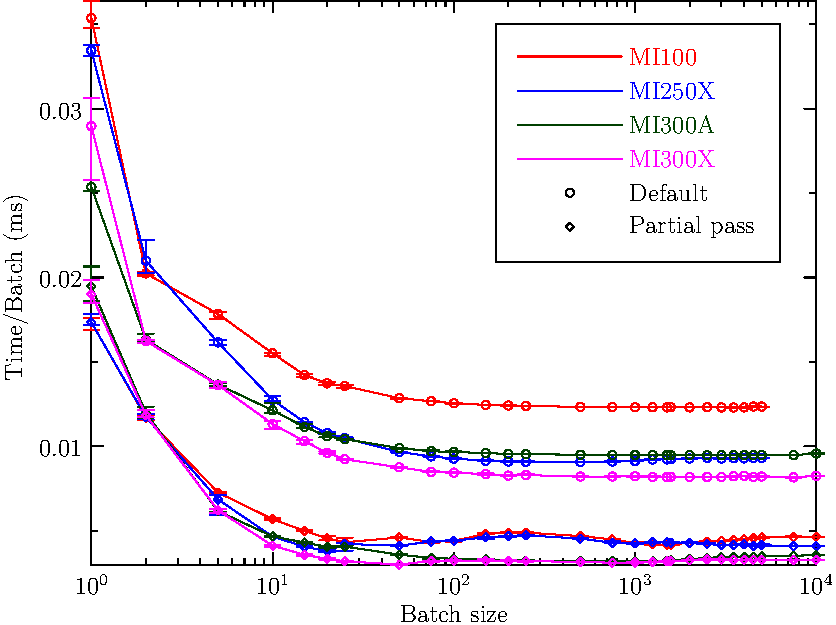
\includegraphics[width=.47\textwidth]{singletime.pdf}} \quad
  \subfloat[$\mkern-90mu$]{\label{subfig:double_precision_time} 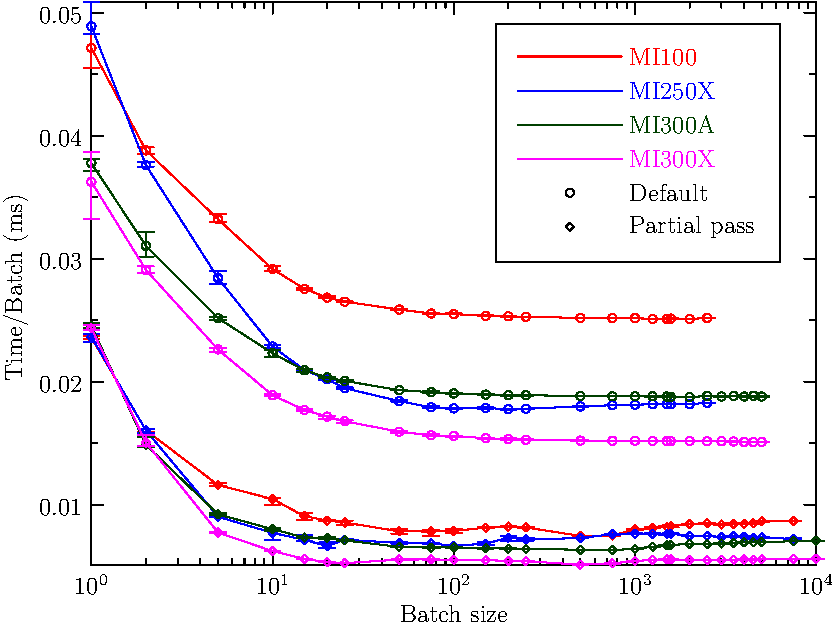
\includegraphics[width=.47\textwidth]{doubletime.pdf}}
  \caption{Median execution time per batch for single-precision (left) and double-precision (right).}
  \label{fig:execution_time}
  \end{figure}
As can be seen in \Cref{fig:execution_time}, the partial-pass
algorithm performs significantly faster than the default
algorithm. For example, in single- and double-precision, the
partial-pass algorithm on MI100, the slower of the tested Instinct accelerators, runs faster than the default algorithm on MI250X, MI300A, and MI300X.

\Cref{fig:speed_up} shows the speedup of partial-pass compared to
default, in single- and double-precision, and batch sizes varying from
$1$ to $10,000$. To compute the speedup, the median execution time
over $50$ runs were used, with 95\% confidence intervals computed by
boot-strap resampling.
\begin{figure}[h]  
    \centering  
    
    \captionsetup[sub]{singlelinecheck=off}
    \subfloat[$\mkern-90mu$]{\label{subfig:single_precision_speedup} 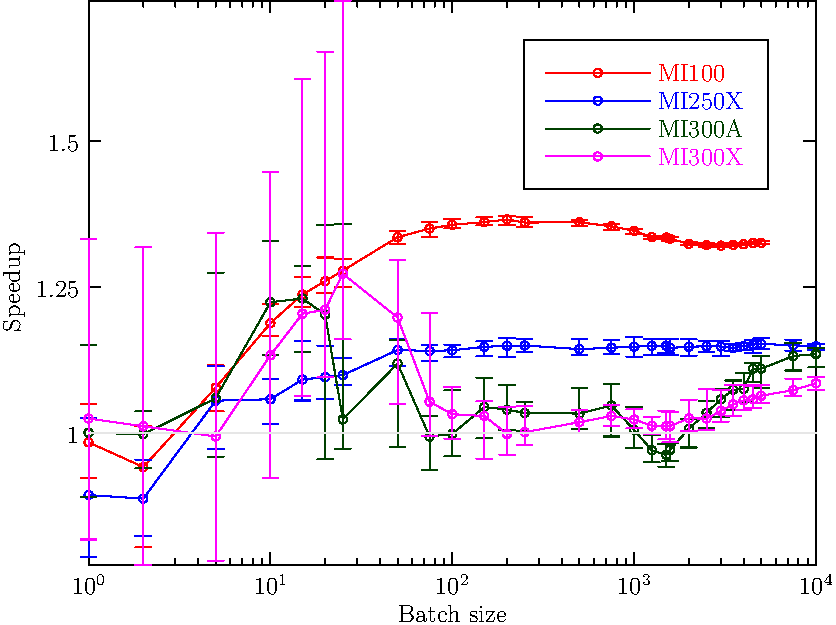
\includegraphics[width=.47\textwidth]{singlespeedup.pdf}} \quad
    \subfloat[$\mkern-90mu$]{\label{subfig:double_precision_speedup} 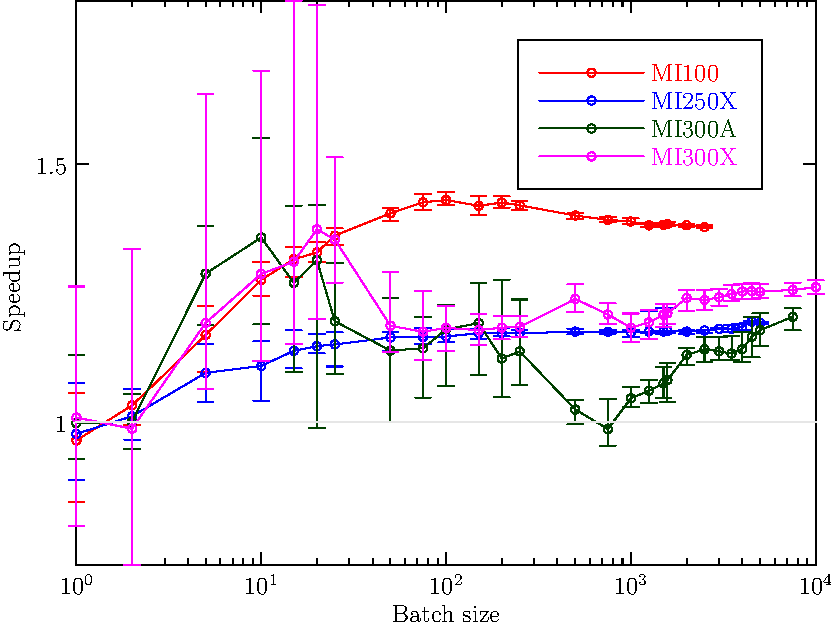
\includegraphics[width=.47\textwidth]{doublespeedup.pdf}}
    \caption{Speedup for single-precision (left) and double-precision (right).}
    \label{fig:speed_up}
  \end{figure}
As can be seen from the results, a significant performance uplift is
achieved with the partial-pass algorithm compared to the default
algorithm. For example, the maximum achievable speedups in
single-precision for MI100, MI250X, MI300A, and MI300X were $1.36$,
$1.51$, $1.23$, and $1.43$, respectively in
\Cref{subfig:single_precision_speedup}. For double-precision in
\Cref{subfig:double_precision_speedup}, the results were up to
$1.43$, $1.92$, $1.36$, and $1.25$ times faster, respectively.

% Bootstrap resampling
% Logarithm y-axis.
% Error bars
% Horizontal line for speed-up 1.

% Base revision: 7406063b
% Partial-pass revision: 57d6d3b6
%
% compute-artifactory.amd.com:5000/rocm-plus-docker/compute-rocm-dkms-no-npi-hipclang:15012-ubuntu-22.04-stg1
%
% ./rocfft-perf run --bench ../../a/clients/staging/dyna-rocfft-bench --lib ~/repo/rocfft/a/library/src/librocfft.so --lib ~/repo/rocfft1/a/library/src/librocfft.so -S partial_pass -o pp/dev -o pp/pp

% asy -f pdf datagraphs.asy  -u'ivariable="batch"' -u 'filenames="data/single/times/mi100dev.mdat,data/single/times/mi100pp.mdat,data/single/times/mi250xdev.mdat,data/single/times/mi250xpp.mdat,data/single/times/mi300adev.mdat,data/single/times/mi300app.mdat,data/single/times/mi300xdev.mdat,data/single/times/mi300xpp.mdat"' -u 'legendlist="MI100,MI250X,MI300A,MI300X,Default,Partial pass"' -o singletime.pdf

% asy -f pdf datagraphs.asy  -u'ivariable="batch"' -u 'filenames="data/double/times/mi100dev.mdat,data/double/times/mi100pp.mdat,data/double/times/mi250xdev.mdat,data/double/times/mi250xpp.mdat,data/double/times/mi300adev.mdat,data/double/times/mi300app.mdat,data/double/times/mi300xdev.mdat,data/double/times/mi300xpp.mdat"' -u 'legendlist="MI100,MI250X,MI300A,MI300X,Default,Partial pass"' -o doubletime.pdf

% asy -f pdf datagraphs.asy  -u'ivariable="batch"' -u 'filenames="data/single/speedup/mi100.sdat,data/single/speedup/mi250x.sdat,data/single/speedup/mi300a.sdat,data/single/speedup/mi300x.sdat"' -u 'legendlist="MI100,MI250X,MI300A,MI300X"' -u"times=false" -o singlespeedup.pdf

% asy -f pdf datagraphs.asy  -u'ivariable="batch"' -u 'filenames="data/double/speedup/mi100.sdat,data/double/speedup/mi250x.sdat,data/double/speedup/mi300a.sdat,data/double/speedup/mi300x.sdat"' -u 'legendlist="MI100,MI250X,MI300A,MI300X"' -u"times=false" -o doublespeedup.pdf

\section{Conclusions and Future Work}

This article presents a new technique for optimizing cache use in multidimensional complex FFTs which require at least three passes.  This
technique involves splitting the calculations along a dimension into two passes;
this allows for the possibility of fitting more calculation into
cache-sized chunks.  For 3D FFTs, this can entirely eliminate a
round-trip to global memory, which results in significantly improved performance in HPC workloads.  While the results presented here are for 3D complex FFTs, we hope to extend this work to multi-kernel 1D and 2D kernels, as well as
real/complex transforms.

\begingroup
\let\itshape\upshape
\bibliographystyle{abbrv}
\bibliography{refs}
\endgroup

%\section*{\st{Acknowledgments}}
%Do \ul{not} include acknowledgments in this blind-review version of the paper, as acknowledgments may provide unintended hints that “deblind” your anonymity. If your paper is accepted to GTAC, the final published version can/should include the appropriate acknowledgments.

\end{document}

% LocalWords:  GTAC FFT rocFFT FFTs ROCm HPC dimensionality radix DFT
% LocalWords:  DFTs GPUs nk eq dft Tukey parallelizable Stockham KiB
% LocalWords:  dimdft strided submatrix Hadamard alg fft amongst GiB
% LocalWords:  dataset subproblem allocatable radices superset im il
% LocalWords:  supersets GROMACS
